% Dokumentation af converter topologi

\chapter{Første Iteration}
I dette afsnit beskrives den indledende og første iteration af designfasen. Den indebærer valg af converter topologi, samt simulering af en ideel converter.

\section{Switch Mode Power-Supply}
I dette projekt vælges der at tage udgangspunkt i Switch Mode Power-Supply (SMPS). Da der er stillet et krav om et maksimalt tab på 5W, betyder det, ved en maksimal udgangseffekt på 75W, at converteren skal have en effektivitet på:
\begin{equation}
	\eta = \frac{75W}{75W + 5W} \cdot 100 = 93.75\percent
\end{equation}

En lineær converter vil ofte have en effektivitet på mellem $30-40\percent$. Da dette ikke vil kunne efterleve kravet på $93.75\percent$, udelukkes de lineære convertere. Dette kan til gengæld tilnærmes ved brug af en SMPS. Ved optimering af tabene i converteren, kan man opnå en effektivitet på op mod $95\percent$\cite{smps}.


\section{Buck Converter}
En simpel converter der bruges til nedregulering af en spænding, er buck converteren. Den består af en transistor, der er placeret i serie med et lavpas filter, i form af et LC-filter. Derudover er der placeret en diode før filteret, således strømmen i spolen har en løbevej, når transistoren går OFF. Det overordnede kredsløb for en buck converter er vist på figur~\ref{fig:buck_converter_circuit}.


\begin{figure}[H]
	\center
	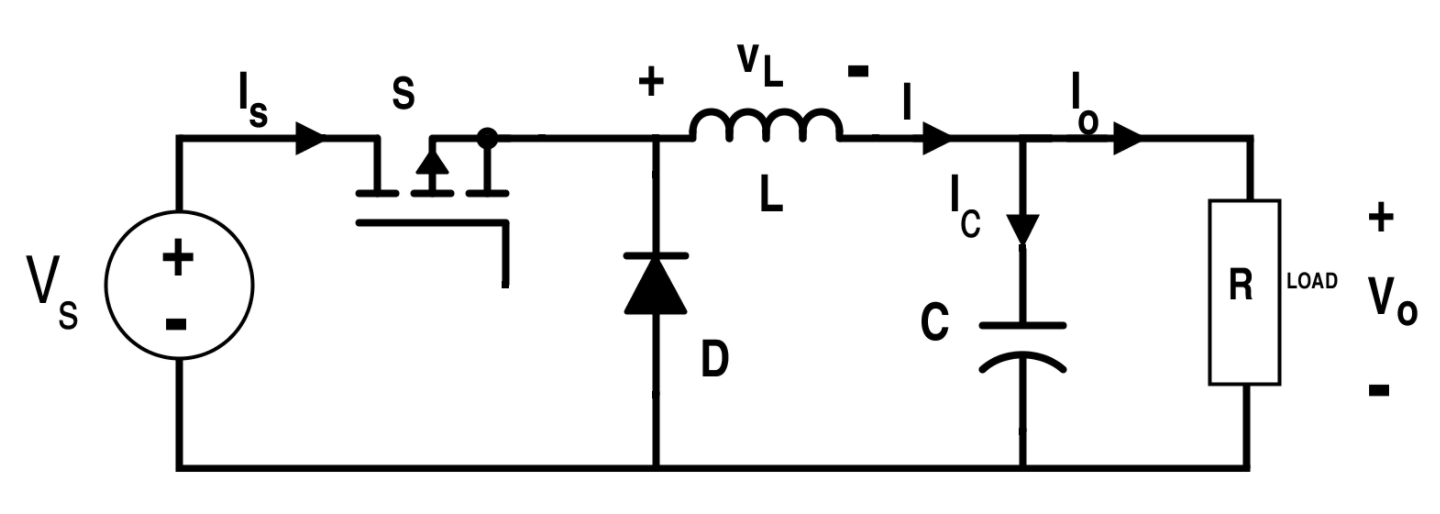
\includegraphics[max width=0.7\linewidth]{/tex/1iteration/billeder/Buck_converter_circuit.PNG}
	\caption{Ideelt diagram af buck converteren
		\cite{buck-converter}}
	\label{fig:buck_converter_circuit}
\end{figure}


I transistorens ON tid, vil strømmen i spolen, og dermed også strømmen i transistoren, rampe op. Det gør den, da der er en positiv spænding over spolen. Den spænding er lig $V_L=V_S-V_O$. Når der er et positivt spændingsfald over spolen, vil dioden være forspændt i spærreretningen, og dermed ikke lede en strøm. Når transistoren går OFF, vil strømmen begynde at løbe gennem dioden, da strømmen i en spole ikke kan skifte momentant. Hvis vi ser dioden som ideel, vil spændingen over spolen nu være lig $V_L=0-V_O$. Da dette giver et negativt spændingsfald over spolen, vil strømmen begynde at aflade i den. Strømmene er skitseret på figur~\ref{fig:buck_converter_current}. Her ses det, at der altid løber en strøm i spolen, mens den skiftes til at løbe i transistoren og dioden, afhængig af ON og OFF perioderne. 


\begin{figure}[H]
	\center
	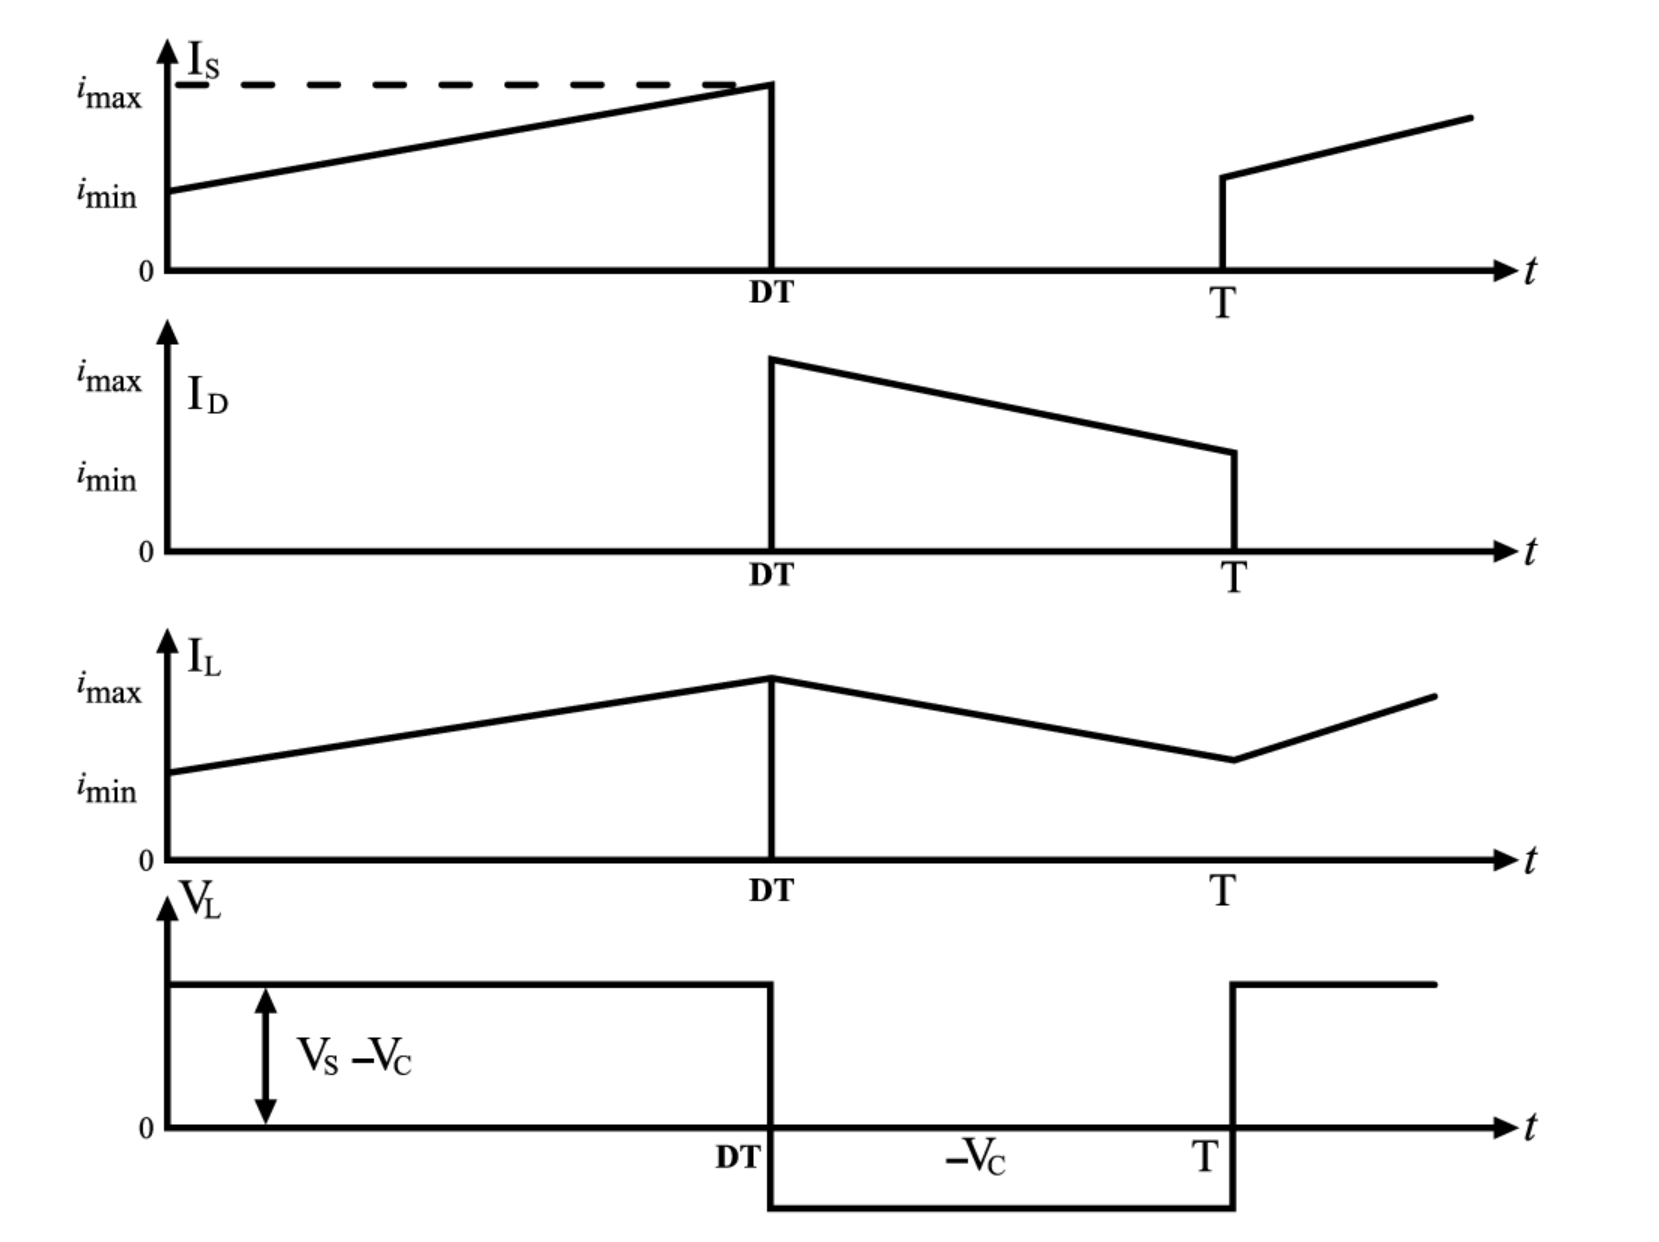
\includegraphics[max width=0.7\linewidth]{/tex/1iteration/billeder/Buck_converter_current.PNG}
	\caption{Buck converter strømme
		\cite{buck-converter}}
	\label{fig:buck_converter_current}
\end{figure}


Da strømmen i spolen aldrig når $0A$, kaldes denne form for operation Continuous Conduction Mode, eller CCM. Overføringsfunktionen for en buck converter i CCM er\cite{SMPS-topologies}:
\begin{equation} \label{buck_converter_overforinsfunktion}
V_{out} = D\cdot V_{in}
\end{equation}

Converteren skal kunne opretholde en outputspænding på $21V$, ved en inputspænding på $26V$. Ved at bruge overføringsfunktionen, regnes den maksimale duty-cycle til ca. $80\percent$. 

En af fordelene ved buck converteren, er at der altid løber en strøm i spolen. Dette gør, at der kan opnås en lille ripple-strøm i filteret, og derved også et mindre tab, både i spolen og kondensatoren. 
En af ulemperne, er at transistoren sidder i den positive forsyningslinje. Dette Kan give komplikationer ved switching af transistoren. Hvis der vælges en p-kanals MOSFET, skal der vælges en PWM-controller der kan håndtere switching af denne. Hvis der vælges en n-kanals MOSFET, skal gate signalet være større end forsyningen, før MOSFET'en er helt ON. Dette kræver flere komponenter, og vil derfor helst undgås. På grund af dette problem undersøges der en converter topologi, hvor MOSFET'en ikke sidder i den positive forsyningslinje.

\section{Flyback Converter}
Flyback converteren, er en transformator baseret topologi. Man deler converteren op i to dele: Primær- og sekundærsiden. Primærsiden består af primærviklingen af transformatoren og en transistor, hvor transistoren fungerer som en switch. Sekundærsiden består af sekundærviklingen, en diode, en udgangskondensator og belastningen. Dette er vist på figur~\ref{fig:flyback_ideal}. En af fordelene ved, at bruge flyback converteren, er at der kan opnås galvanisk adskillelse mellem primær- og sekundærsiden af transformatoren, samt MOSFET'ens source er forbundet til GND. Derudover bruges der det samme antal komponenter, som ved buck converteren.

\begin{figure}[H]
	\center
	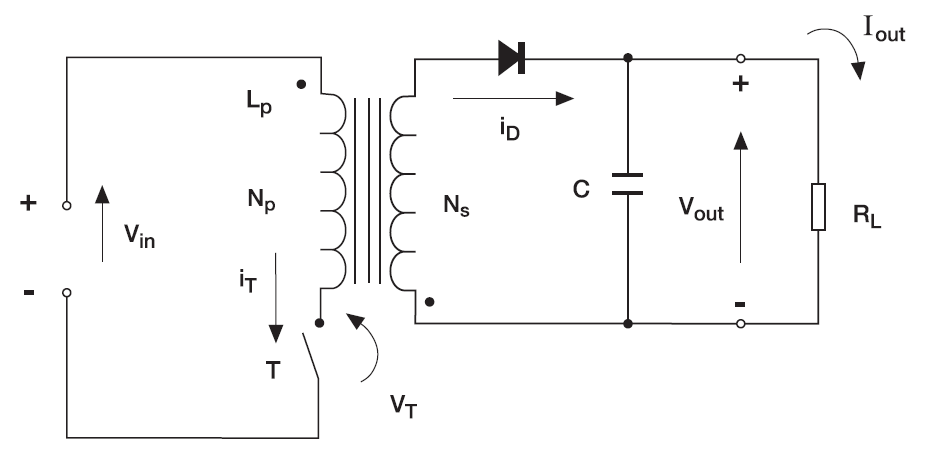
\includegraphics[max width=0.7\linewidth]{/tex/1iteration/billeder/flyback_ideal.PNG}
	\caption{Ideelt diagram af flyback converteren
	\cite{SMPS-topologies}}
	\label{fig:flyback_ideal}
\end{figure} 

\noindent Flyback converteren bruges til at konvertere en indgangsspænding, ned til en mindre udgangsspænding. Dette gøres ved at styre transistoren med et PWM-signal, med en variabel duty-cycle. Når den er ON, vil der være en positiv spænding ved prik-enden af viklingen ift. den anden ende. Ud fra formlen $V=L\cdot \frac{di}{dt}$ kan det ses, at når der ligger en spænding over viklingen, vil strømmen i transformatoren stige lineært, over den tid transistoren er ON. Når transistoren går OFF, vil den magnetiske strøm i transformatoren inducere en spænding over sekundærviklingen. Når denne spænding bliver lig udgangsspændingen, vil dioden begynde at lede den strøm, der er oplagret i transformatoren. Da spændingen over sekundærviklingen er positiv ved prikken, og dermed modsat af primærviklingen, vil strømmen falde lineært ud fra samme forhold, som nævnt tidligere. Dette vil over tid skabe en trekantet kurveform af den samlede strøm i transformatoren. Et eksempel på dette kan ses på figur \ref{fig:CCM_transformer_current}. Da strømmen i hver vikling er diskontinuert, vil det give anledning til større peak-strømme. Det er maksimalt $50\percent$ af tiden der løber en strøm i viklingen, hvilket betyder en større strøm for at opretholde den samme middelstrøm.

Flyback converteren kan overordnet drives på to forskellige måder, Continuous Conduction Mode (CCM) og Discontinuous Conduction Mode (DCM). Disse to måder har forskellige fordele og ulemper, som skal tages højde for inden der vælges hvordan converteren skal drives. 

\subsection{Continuous Conduction Mode}
Forkellen ved CCM og DCM er, hvordan strømmen løber i transformatoren. Ved CCM vil der altid løbe en strøm i transformatoren, som der også ligger i navnet. Dog vil strømmene individuelt i viklingerne være diskontinuerte. Strømmen er skitseret på figur \ref{fig:CCM_transformer_current}. Skal man have den samlede strøm i transformatoren, skal de to kurver for primær- og sekundærviklingen samles. Dette er fordi der kun løber en strøm i primærviklingen når transistoren er ON, og en strøm i sekundærviklingen når transistoren er OFF. 

\noindent Overføringsfunktionen for en flyback converter i CCM er\cite{SMPS-topologies}:
\begin{equation} \label{flyback_converter_CCM_overforinsfunktion}
V_{out} = \frac{N_S}{N_P} \cdot \frac{D}{1-D} \cdot V_{in}
\end{equation}
Ud fra overføringsfunktionen ses det, at udgangsspændingen både afhænger af duty-cyclen, og af omsætningsforholdet i transformatoren. 

\begin{figure}[H]
	\center
	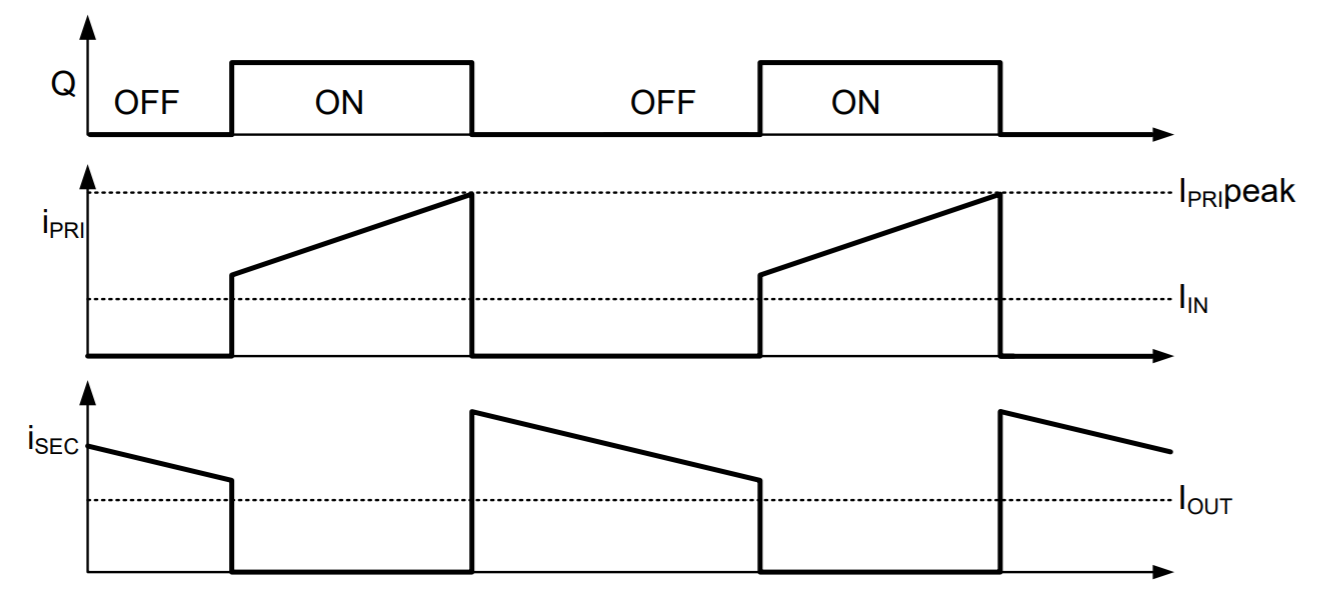
\includegraphics[max width=0.7\linewidth]{/tex/1iteration/billeder/CCM_transformer_current.PNG}
	\caption{CCM transformator strømme
	\cite{SMPS-topologies}}
	\label{fig:CCM_transformer_current}
\end{figure}

\noindent En af fordelene ved CCM er, at strømmen i transformatoren ikke når at aflade helt, inden transistoren går ON igen. Dette giver lavere ripple-strømme, og dermed også peak-strømme, hvilket giver anledning til et mindre effekttab. På grund af den mindre ripple-strøm i transformatoren, opnås der også en mindre ripplespænding på udgangen. hvilket sætter et mindre krav til udgangskondensatoren. 

\subsection{Discontinuous Conduction Mode}
Den anden måde at drive converteren på er DCM. Ved denne metode vil der være en død tid i hver periode, hvor der ikke løber en strøm i transformatoren. Dette betyder at transformatoren når at aflade helt, inden switch-perioden er ovre. Til forskel fra CCM, vil dette give nogle trekantede strømkurver i transformatoren, som ses på figur~\ref{fig:DCM_transformer_current}.
På grund af død tiden, vil peak-strømmene blive større, da arealet under kurven skal være det samme som ved CCM, for at kunne opretholde den samme udgangsstrøm. 
Fordelen ved at $di$ bliver større, er at induktansen i viklingerne bliver mindre. Tilgengæld giver det anledning til større tab, da både peak- og ripple-strømmene bliver større.

\begin{figure}[H]
	\center
	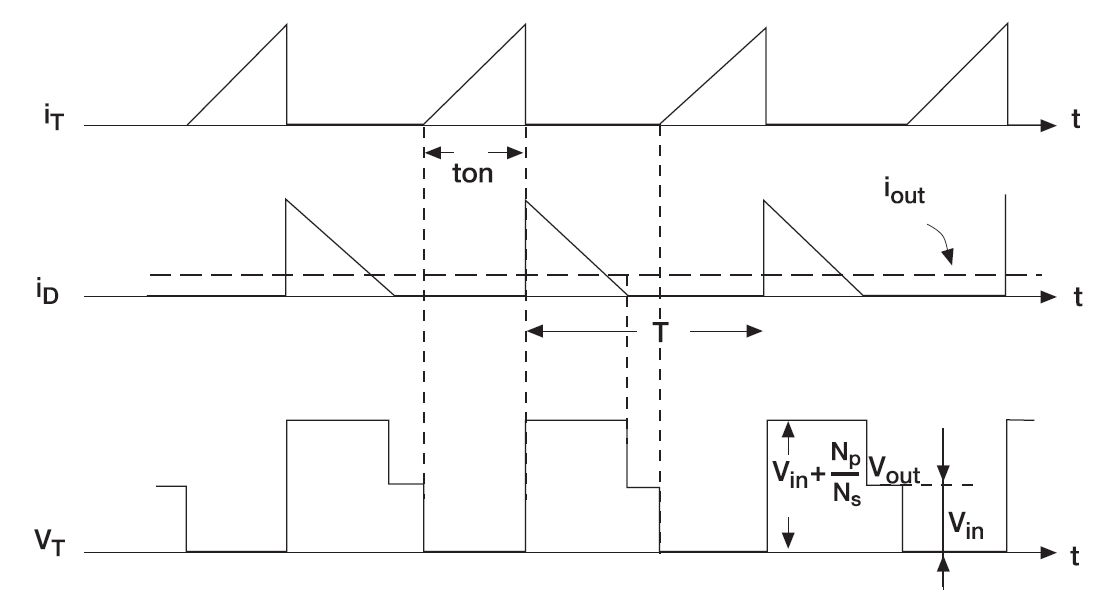
\includegraphics[max width=0.7\linewidth]{/tex/1iteration/billeder/DCM_transformer_current.PNG}
	\caption{DCM transformator strømme
		\cite{SMPS-topologies}}
	\label{fig:DCM_transformer_current}
\end{figure}

Overføringsfunktionen for flyback converteren i DCM er\cite{SMPS-topologies}:
\begin{equation} \label{flyback_converter_DCM_overforinsfunktion}
V_{out} = \frac{N_S}{N_P} \cdot \frac{D}{1-D} \cdot V_{in}
\end{equation}



\section{Ideel transformator}
Der vælges at arbejde videre med en flyback converteren, pga. komplikationerne ifm. switchingen af MOSFET'en ved buck converteren.
Der regnes strømme i transformatoren for både CCM og DCM, for derefter, at vurdere forskellene mellem de to metoder.

Der tages udgangspunkt i en converter der, ved en input spænding på $26V-50V$, skal kunne opretholde en udgang på $21V$ og $2.5A$. Derudover antages det at transformatoren har et omsætningsforhold på 1.

\subsection{CCM}
Først beregnes den maksimale og minimale duty-cycle:
\begin{equation} \label{D_maks_CCM}
D_{maks} = \frac{V_{out}}{V_{inmin} + V_{out}} = 0.447
\end{equation}
\begin{equation} \label{D_min_CCM}
D_{min} = \frac{V_{out}}{V_{inmaks} + V_{out}} = 0.174
\end{equation}

\noindent Nu kan de maksimale ripple-, peak- og RMS-strømme i transformatoren estimeres. 
\begin{equation} \label{I_ripple_CCM}
I_{ripple} = 0.6 \cdot \frac{V_{out} \cdot I_{out}}{V_{inmaks} \cdot   D_{min}} = 2.13A
\end{equation}
\begin{equation} \label{I_pk_CCM}
I_{pk} = \frac{V_{out} \cdot I_{out}}{V_{inmin} \cdot D_{maks}} + \frac{I_{ripple}}{2} = 5.58A
\end{equation}
\begin{equation} \label{I_pk_avg_CCM}
I_{pkavg} = \frac{I_{out}}{1-D_{maks}} = 4.52A
\end{equation}

\noindent Nu beregnes RMS-strømmene i både primær- og sekundærviklingerne. 
\begin{equation} \label{I_p_RMS_CCM}
I_{RMSp} = \sqrt{D_{maks} \cdot (I_{pkavg})^2} = 3.02A
\end{equation}
\begin{equation} \label{I_s_RMS_CCM}
I_{RMSs} = \sqrt{(1-D_{maks}) \cdot (I_{pkavg})^2} = 3.36A
\end{equation}

Induktansen i primærviklingen beregnes ud fra den ønskede ripplestrøm, samt switch-frekvensen. Som udgangspunkt vælges den til $100kHz$. Fordi omsætningsforholdet i transformatoren er lig 1, betyder det at $L_p = L_s$.
\begin{equation} \label{L_CCM}
L = \frac{V_{inmin} \cdot D_{min}}{I_{ripple} \cdot f_s} = 69.43\micro H
\end{equation}

\subsection{DCM}
Nu foretages strøm beregninger for en flyback converter i DCM.
Da overføringsfunktionen for CCM og DCM er den samme, betyder det både den maksimale og minimale duty-cycle er ens ved de to.
Derfor startes der med at regne peak-strømmen. Strømmen regnes ved det der kaldes boundary, som er det punkt hvor transformatoren lige præcis når at aflade i en switch-periode.
\begin{equation} \label{DCM_peak_current}
I_{pk} = I_o \cdot \frac{2}{1-D_{maks}} = 9.04A
\end{equation}

Da transformatoren når at aflade ved DCM er ripple-strømmen lig peak-strømmen:
\begin{equation} \label{DCM_ripple_current}
I_{ripple} = I_{pk} = 9.04A
\end{equation}

Induktansen i primærviklingen beregnes igen ud fra ligning~\ref{L_CCM}. Da peak-strømmen, og dermed også ripple-strømmen er regnet ved boundary, betyder det at der regnes en maksimal induktans, for hvor converteren stadig operer i DCM.
\begin{equation} \label{L_DCM}
L = \frac{V_{inmin} \cdot D_{min}}{I_{ripple} \cdot f_s} = 12.85\micro H
\end{equation}

Da induktansen er en maksimal værdi, skal man ligge med en hvis margin til denne, for at sikre, at converteren operer i DCM. Hvis induktansen i viklingerne mindskes, vil man opnå en større peak-strøm i transformatoren. Med en ripple-strøm på minimum $9.04A$, vurderes det at effekttabene ved at operere i DCM, vil blive for store. Derfor vil der fremadrettet arbejdes videre med en flyback converter i CCM.


\section{Udgangskondensator}
I en flyback converter bruges udgangskondensatoren primært til at mindske ripplespændingen på load'en. Formlen for at beregne minimumskapaciteten er
\begin{equation} \label{udgangskondensator}
C_{out} \geqslant \frac{I_{out} \cdot D_{maks}}{V_{ripple} \cdot f_s} \geqslant 223.4 \micro F
\end{equation}

\section{Simulering}
Med udgangspunkt i figur~\ref{fig:flyback_ideal} opsættes en ideel flyback converter i p-spice. Dette er gjort på figur~\ref{fig:ideal_flyback_diagram}. Converteren er sat op med en ideel transformatorkobling, et ideelt switching element, samt en ideel diode, for at få et indblik i flyback converterens virkemåde. 


\begin{figure}[H]
	\center
	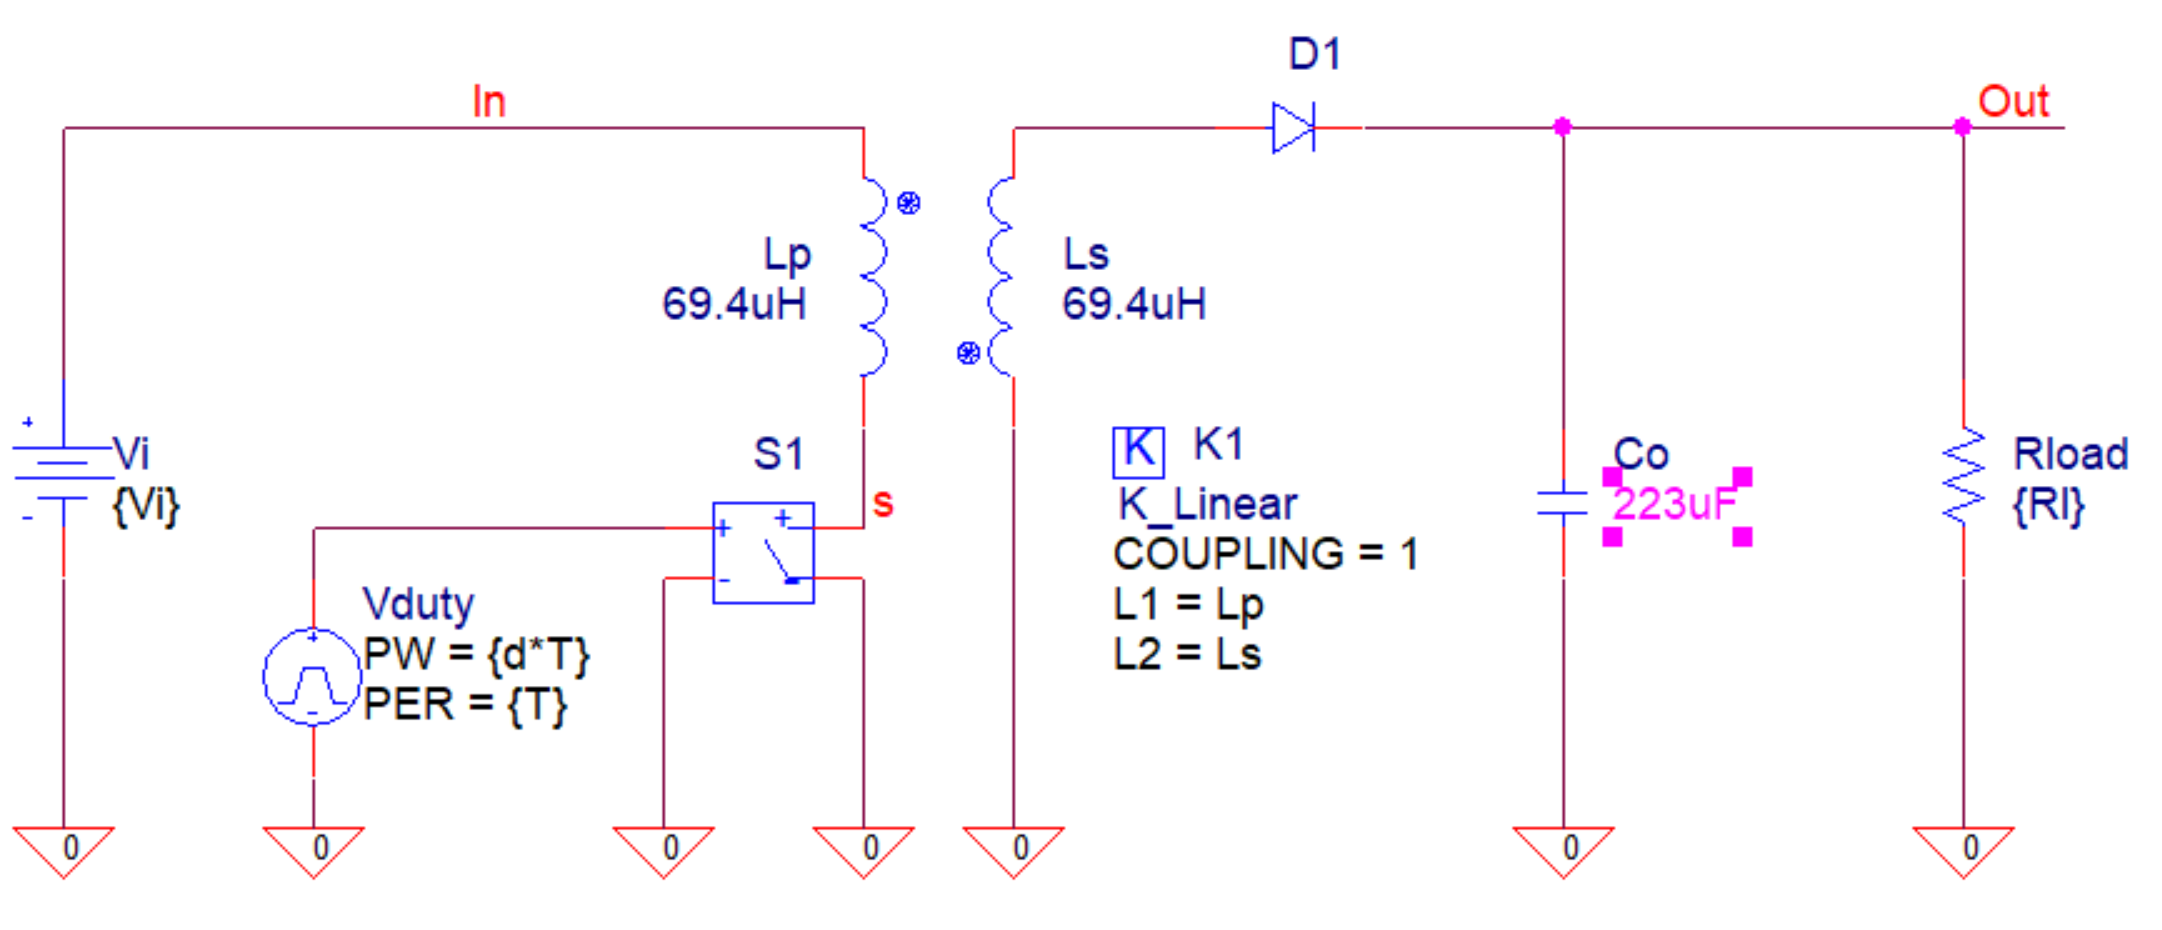
\includegraphics[max width=0.7\linewidth]{/tex/1iteration/billeder/flyback_ideal_diagram.PNG}
	\caption{Ideelt flyback kredsløb}
	\label{fig:ideal_flyback_diagram}
\end{figure}

Der er to scenarier der er relevante at kigge på, ved en indgangsspænding på $26V$, samt ved en indgangsspænding på $50V$. Først kigges der på udgangen af converteren, for at kontrollere udgangsstrømmen og -spændingen. På figur~\ref{fig:26V_ideal_output} ses både outputstrømmen (rød) og -spændingen (grøn), med en inputspænding på 26V. Her ses det at spændingen ligger sig omkring $21V$ og strømmen ligger sig omkring $2.5A$, hvilket var kravet til converteren. Derudover aflæses ripplespændingen til ca. $50mV$, hvilket er overholder kravet for ripplespændingen. 

\begin{figure}[H]
	\center
	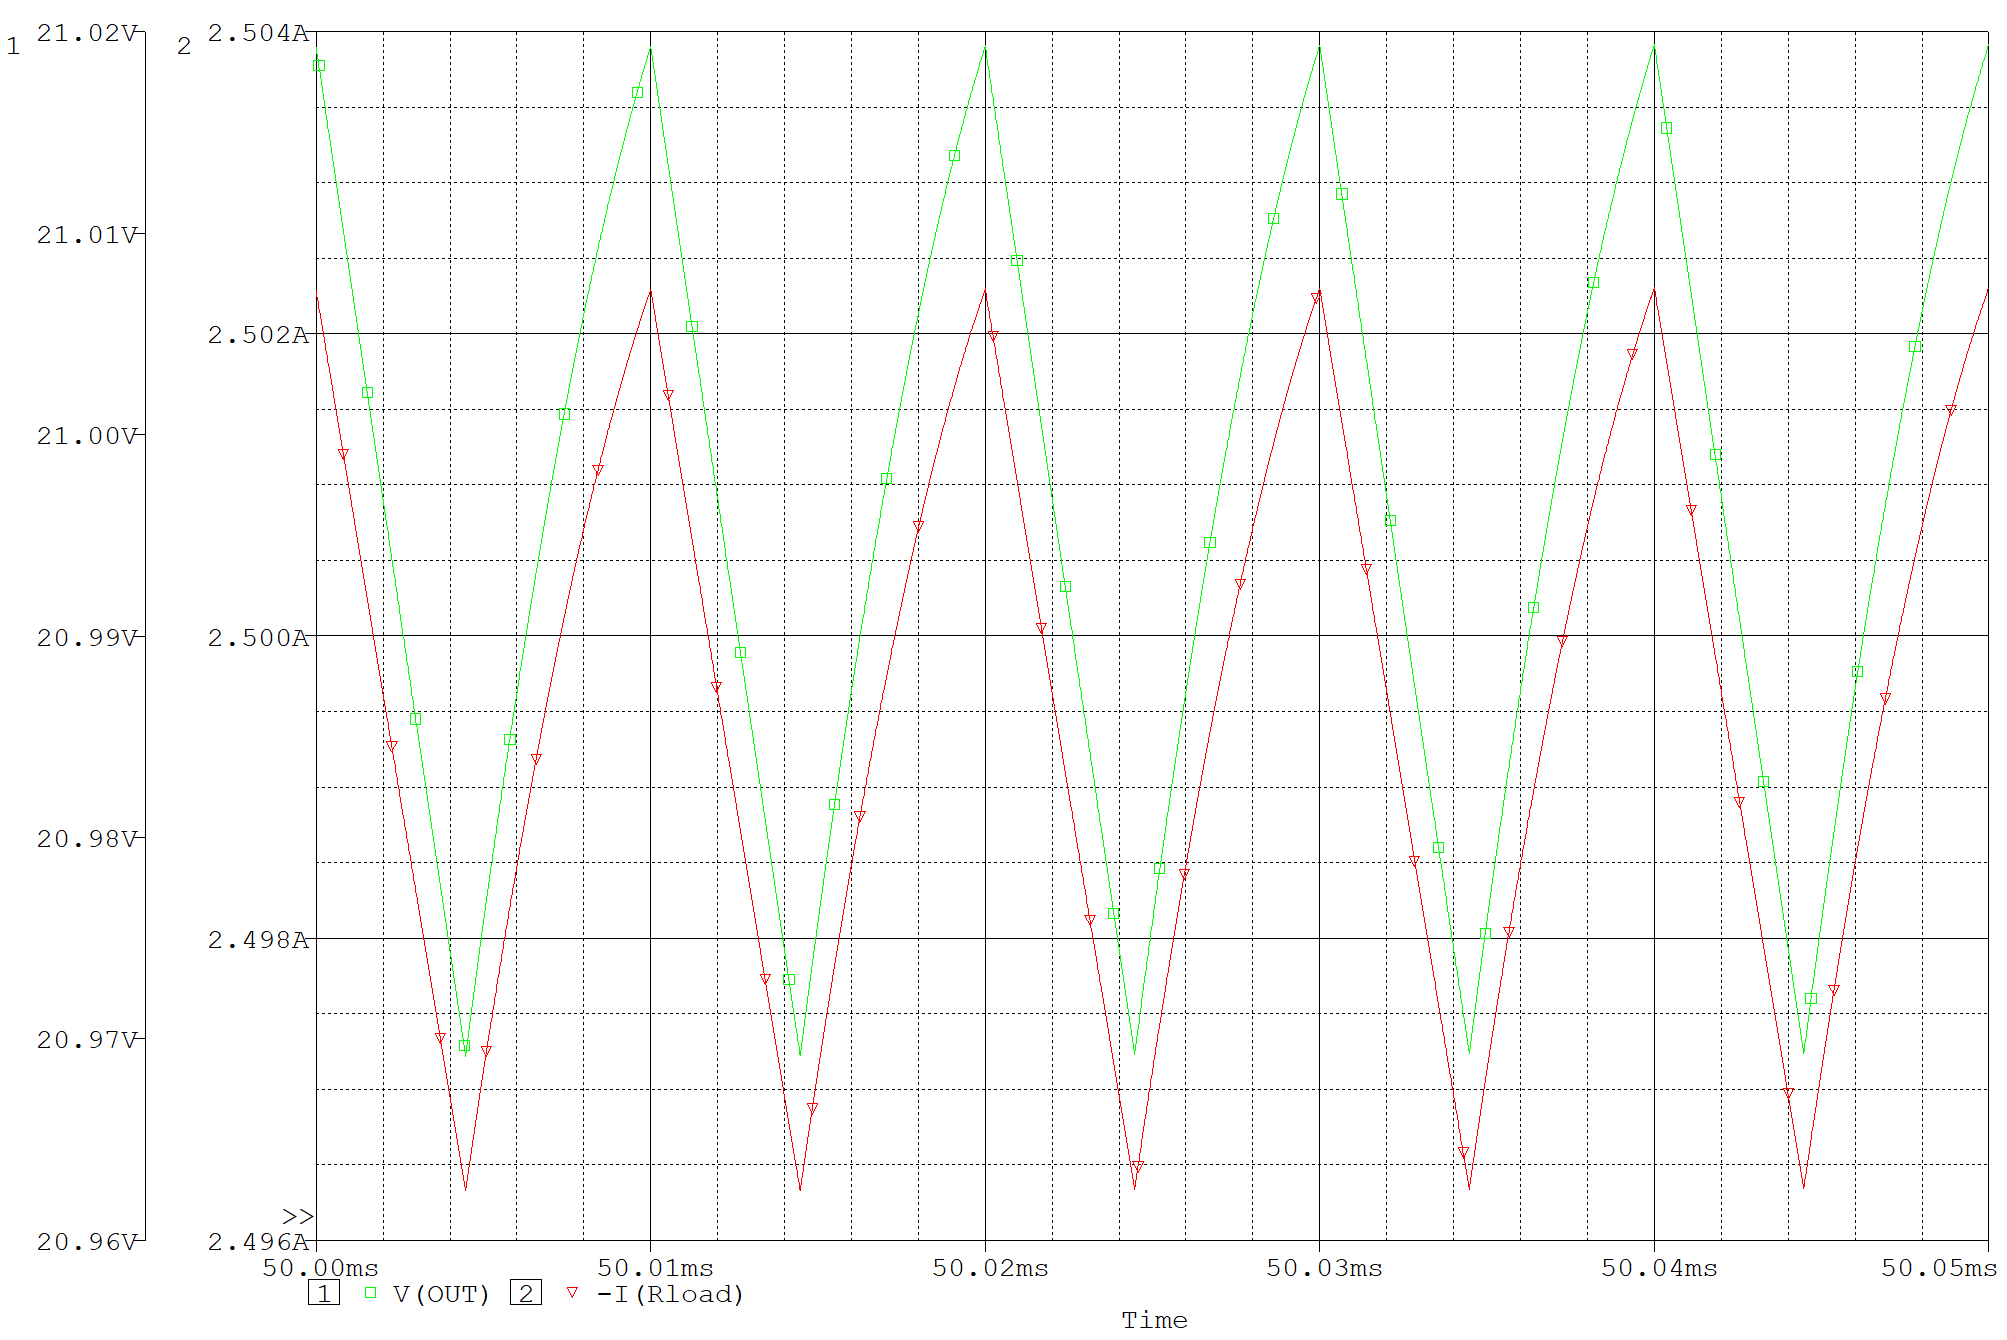
\includegraphics[max width=0.7\linewidth]{/tex/1iteration/billeder/26V_output.PNG}
	\caption{Converter output - ved 26V input}
	\label{fig:26V_ideal_output}
\end{figure}

\noindent På figur~\ref{fig:50V_ideal_output} ses det samme billede, ved $50V$ inputspænding. Da converterens duty-cycle er faldet, falder ripple-spændingen også. Den aflæses til ca. $33mV$. 


\begin{figure}[H]
	\center
	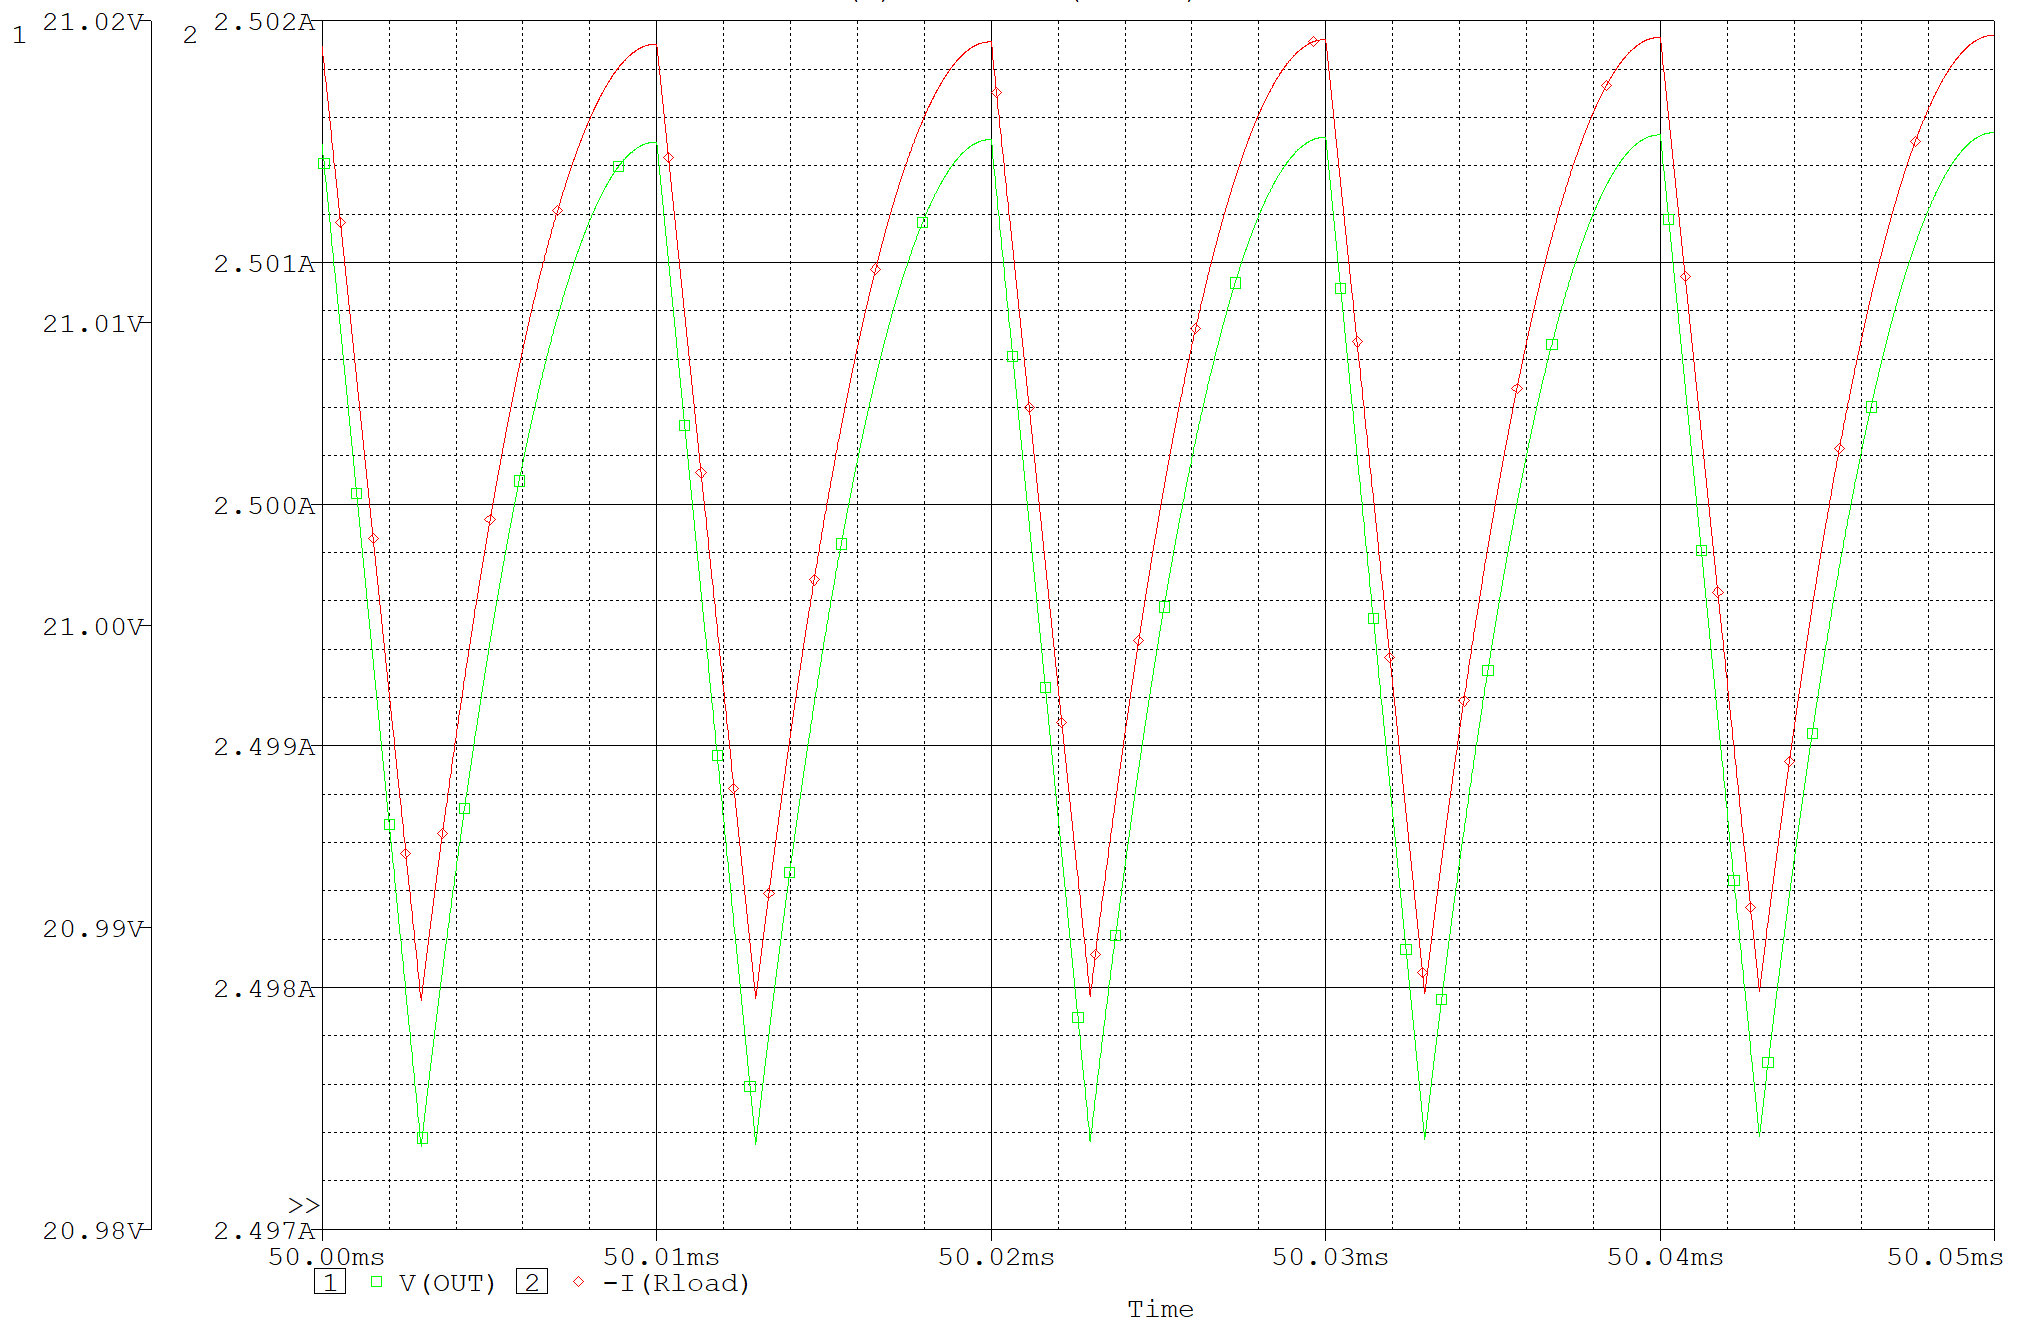
\includegraphics[max width=0.7\linewidth]{/tex/1iteration/billeder/50V_output.PNG}
	\caption{Converter output - ved 50V input}
	\label{fig:50V_ideal_output}
\end{figure}

\noindent I tabel~\ref{tab:result_ideal_converter} ses resultaterne for analyse(A) og simulering(S), af den ideelle converter. Ripple- og peak-strømmene er aflæst ud fra figur~\ref{fig:26V_transformer_current} og \ref{fig:50V_transformer_current}. RMS-strømmene findes ved, at bruge RMS-funktionen i p-spice. Derudover kan det konstateres at converteren operer i CCM, da transformatorstrømmen ikke når at aflade helt. Se figur~\ref{fig:CCM_transformer_current}. 

\begin{table}[H] 			
	\centering
	\begin{tabularx}{\textwidth}{|X|c|c|c|c|c|c|c|c|}
		\hline
		\textbf{Indgangs-spænding} & \multicolumn{2}{|X|}{\textbf{Ripple-strøm}} & \multicolumn{2}{|X|}{\textbf{Peak-strøm}} & \multicolumn{2}{|X|}{\textbf{RMS-strøm i primær}} & \multicolumn{2}{|X|}{\textbf{RMS-strøm i sekundær}} \\ \hline
		& A & S & A & S & A & S & A & S \\ \hline
		$26V$ & $1.67A$ & $1.66A$ & $5.36A$ & $5.35A$ & $3.02A$ & $3.08A$ & $3.36A$ & $3.33A$ \\ \hline 
		$50V$ & $2.13A$ & $2.11A$ & $4.62A$ & $4.61A$ & $1.93A$ & $1.98A$ & $2.98A$ & $3.01A$ \\ \hline
	\end{tabularx}
	\caption{Resultater for analyse og simulering af ideel flyback converter}
	\label{tab:result_ideal_converter}
\end{table}

\begin{figure}[H]
	\center
	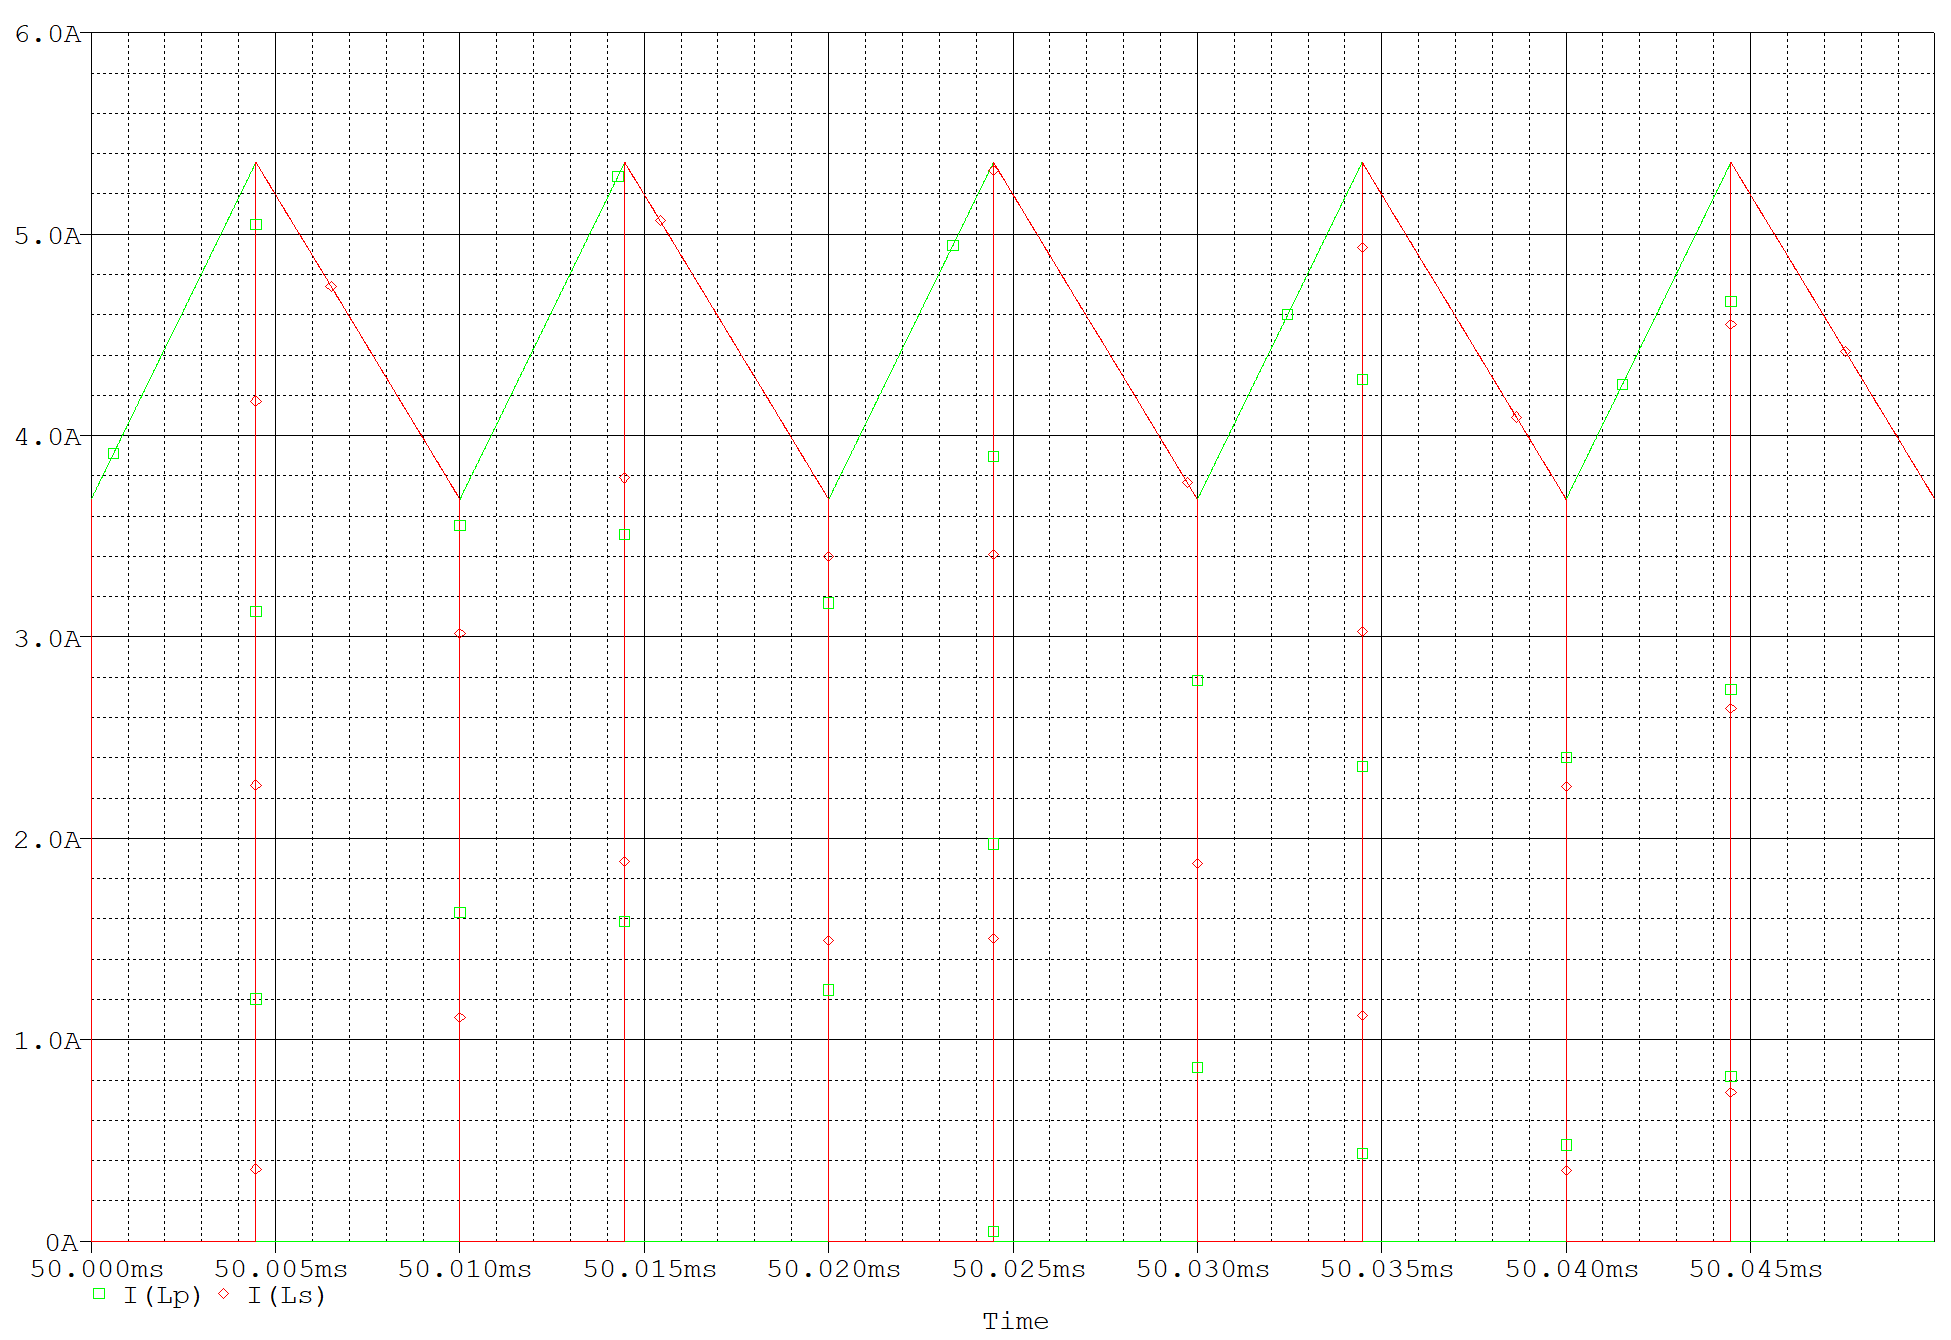
\includegraphics[max width=0.7\linewidth]{/tex/1iteration/billeder/26V_transformer_current.PNG}
	\caption{Transformator strømme - ved 26V input}
	\label{fig:26V_transformer_current}
\end{figure}

\begin{figure}[H]
	\center
	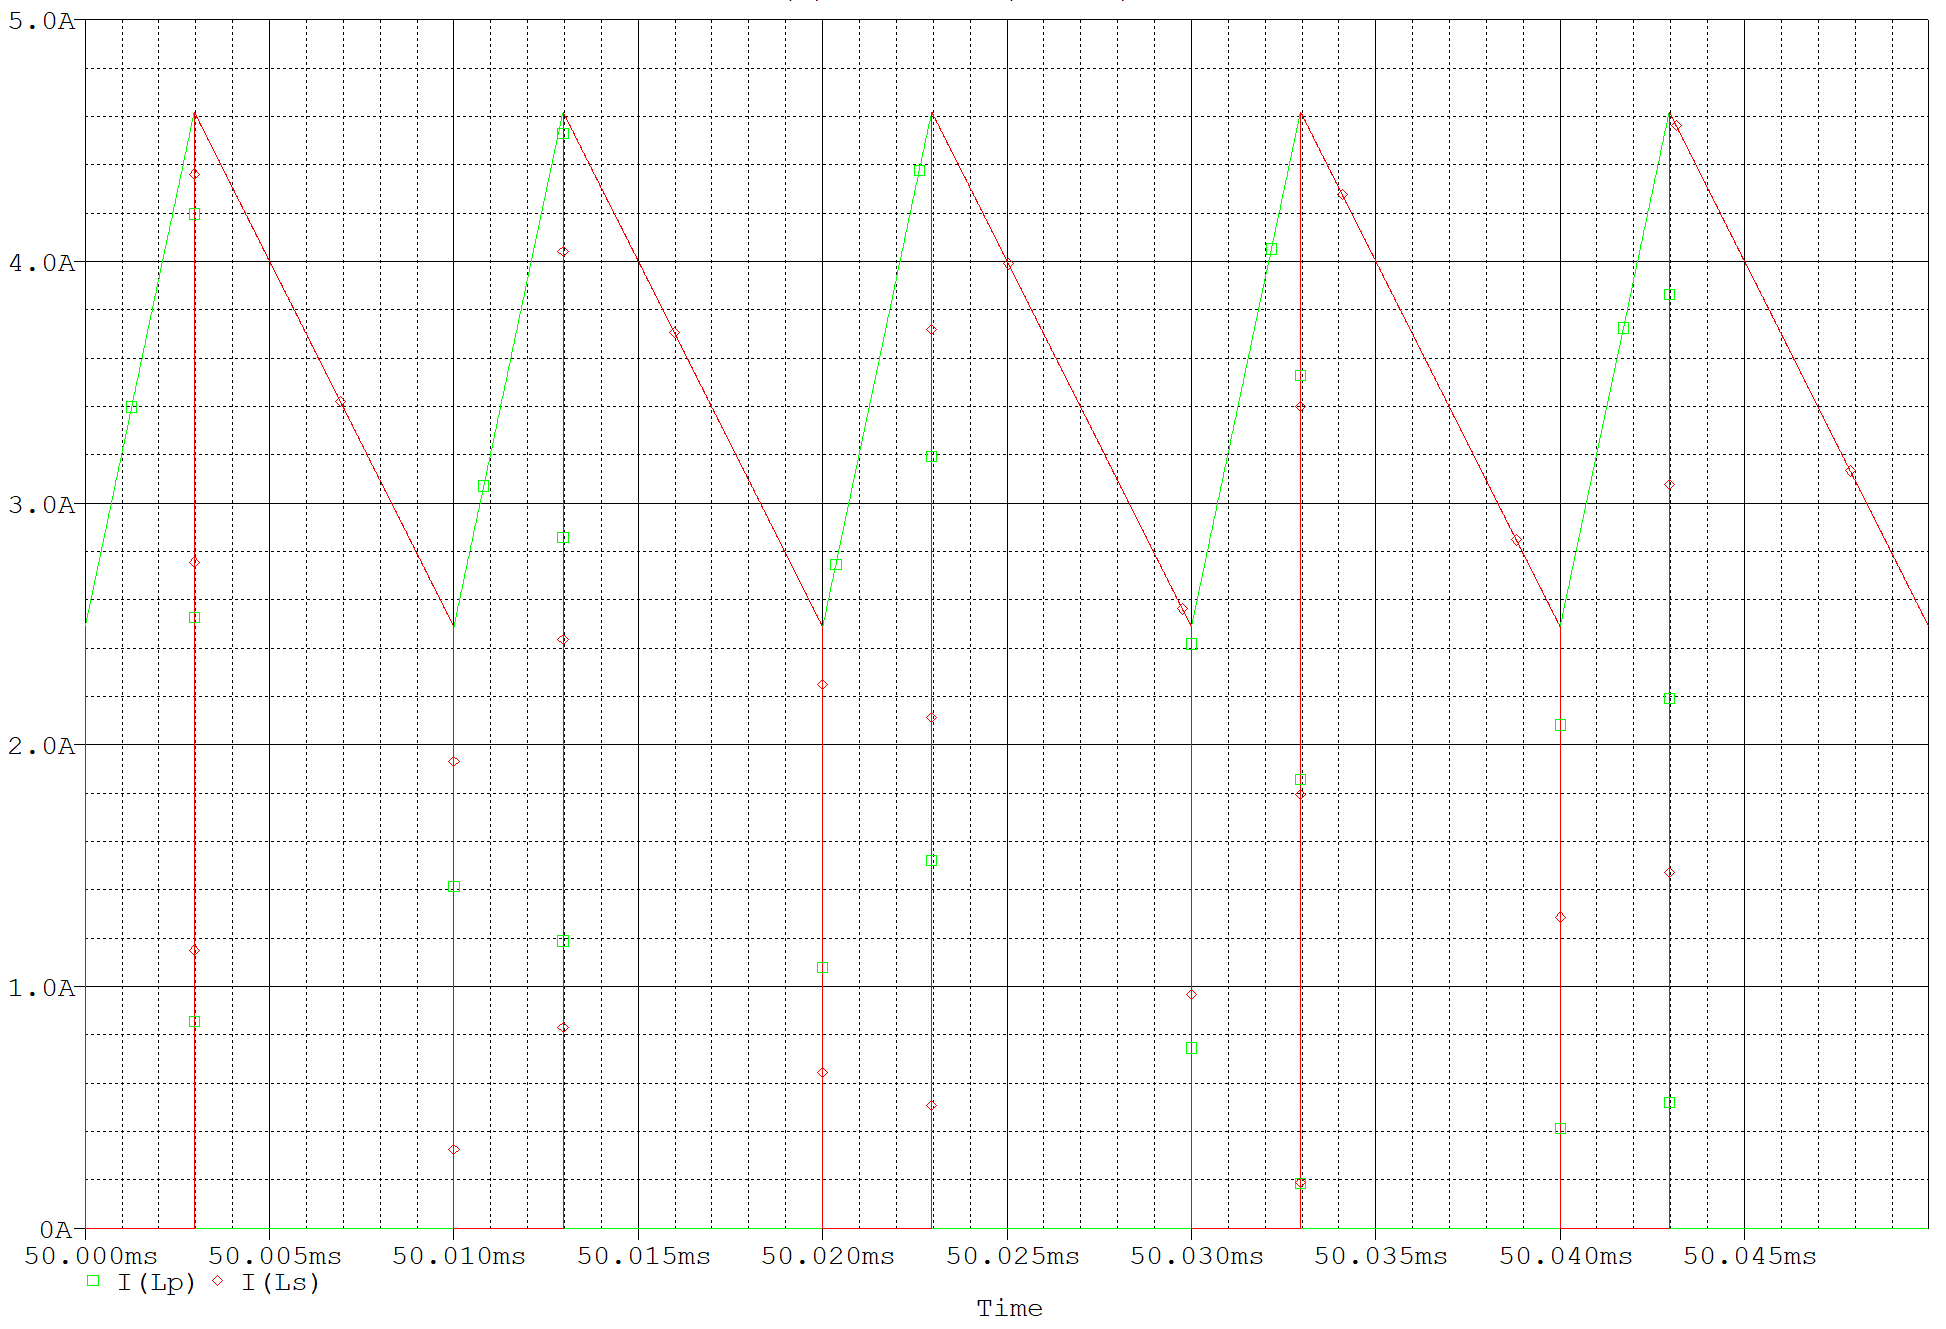
\includegraphics[max width=0.7\linewidth]{/tex/1iteration/billeder/50V_transformer_current.PNG}
	\caption{Transformator strømme - ved 50V input}
	\label{fig:50V_transformer_current}
\end{figure}



